% !TEX root = ../../STP_IoTjournal.tex
\subsection{High UAV Density with $6$ m/s Wind \label{sec:city_simResults}}
As per Algorithm \ref{alg:rtt}, we start with $\veh_1$ and sequentially compute the optimal control policy $\tracklaw_j$ and the latest departure time $\ldt_j$ for each vehicle. To compute the error bound $\errorbound_j$ on the tracking error of vehicle $j$, we choose $R_{\text{EB}} = 5$ m and use the reduced control authority $\cset^p_j = \{(v_{r,j}, \omega_{r,j}): 11 \text{ m/s} \leq v_{r,j} \leq 13 \text{ m/s}, |\omega_{r,j}| \leq 1.2 \text{ rad/s}\}$. Given dynamics in \eqref{eq:dyn_i}, the error dynamics between $\veh_j$ and the virtual evader are given by \cite{Mitchell05}:
\begin{equation}
\label{eq:reldyn}
\begin{aligned}
\dot{e}_{x,j} &= v_{j} \cos(e_{\theta,j}) - v_{r,j} + \omega_{r,j}{e}_{y,j} + d_{x,j}\\
\dot{e}_{y,j} &= v_{r,j}\sin(e_{\theta,j}) - \omega_{r,j}{e}_{x,j} + d_{y,j}\\
\dot{e}_{\theta,j} &= \omega_{j} - \omega_{r,j},
\end{aligned}
\end{equation}    
where $e_j = ({e}_{x,j}, {e}_{y,j}, {e}_{\theta,j})$ is the tracking error in the three states of $\veh_j$. Given relative dynamics, we compute the BRS $\brs^{\text{EB}}$ using \eqref{eqn:errBound} and evaluate the infinite-horizon control invariant set $\disckernel_j$. For all the BRS computations in this simulation, we use Level Set Toolbox \cite{Mitchell07b}. In presence of moderate winds, the obtained tracking error bound is $5$ m. This means that given any trajectory (which is a sequence of states over time) of vehicle, winds can at most cause a deviation of $5$ m from this trajectory at all times. Consequently, the vehicle will be within a distance of $5$ m from the trajectory. Note that since all STP vehicles have same dynamics, the error bound is also same for all vehicles. 

The optimal control policy for $\veh_j$ is thus given by $\tracklaw_j(e_j)$ in \eqref{eq:robust_tracking_law}. However, to compute the relative state $e_j$, the nominal trajectory $\state_{r,j}$ for $\veh_j$ is required. Using $\disckernel_j$, we compute the obstacles induced by the higher-priority vehicles for $\veh_j$ and the obstacle induced by $\veh_j$ for the lower-priority vehicles. These obstacles are given by \eqref{eqn:rttAugObs} and \eqref{eqn:rttObs} respectively. Note that since disturbance directly impacts the computation of tracking error bound, these obstacles also grow as disturbance magnitude increases. We will illustrate the effect of disturbance magnitude on the trajectories of vehicles in \ref{sec:city_sim}-\ref{sec:city_distbEffect}.

The nominal trajectory can now be obtained by computing $\brs_j^\text{rtt}$ in \eqref{eq:rttBRS} and executing the corresponding control policy $\ctrl_j^\text{rtt}$ in \eqref{eq:RTTOptCtrl}, starting from the initial state $\state^0_j$. Finally, the latest departure time $\ldt_j$ is given by $\arg \sup_t \state^0_j \in \brs_j^\text{rtt}(t, \sta_j)$. It is important to note that since the BRS $\brs_j^\text{rtt}$ is computed backwards starting from the scheduled time of arrival $\sta_j$, (a) the latest departure time $\ldt_j$ directly depends on and varies with $\sta_j$ and (b) it directly impacts the obstacles that $\veh_j$ needs to avoid in its trajectory towards its destination. We will illustrate the effect of the scheduled time of arrival on the trajectories of vehicles also in \ref{sec:city_sim}-\ref{sec:city_distbEffect}.

The resulting trajectories of vehicles for $d_{r} = 6$ m/s and $\sta_j = 0 ~ \forall j$ at different times are shown in Figure \ref{fig:trajectories_sf_snapshots}. As evident from the figures, the vehicles remain clear of all the static obstacles (the black contours) and make steady progress towards reaching their destinations. The vehicles whose destinations are relatively closer need less time to travel to their destinations and depart later. Note that the shown trajectories are simulated under uniformly random disturbance (i.e., for every vehicle, the disturbance is uniformly sampled from a circle of radius $d_{r} = 6$ m/s at each time step), but the STP algorithm guarantees safety and reactivity despite the worst case disturbance, as we show later in this section.
%
\begin{figure*}[!htb]
 \centering
\begin{subfigure}{0.5\textwidth}
  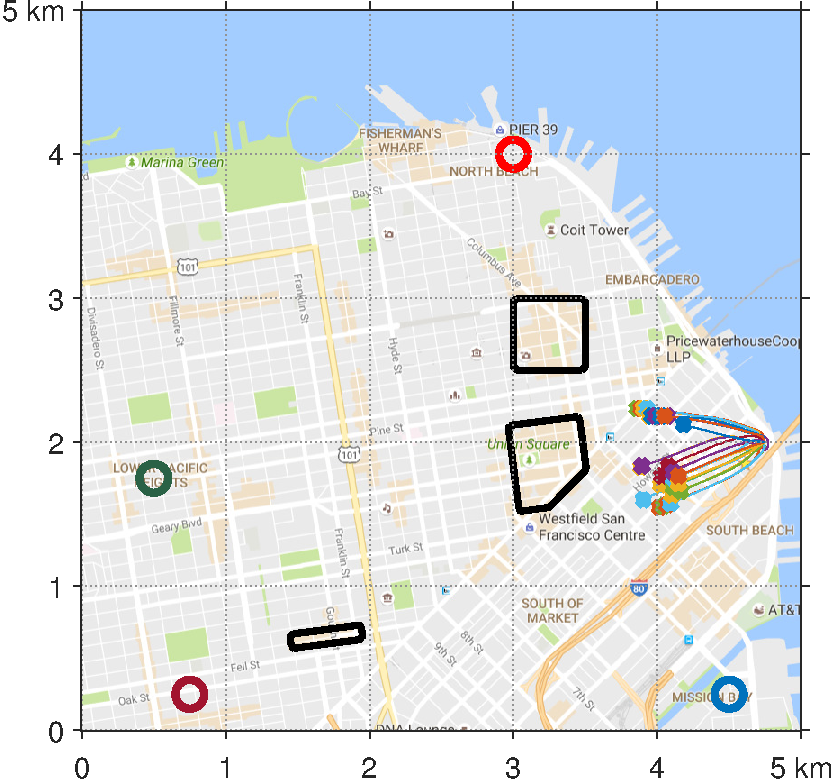
\includegraphics[width=\columnwidth]{figs/sf_d6sep0_s1}
  \subcaption{}
  \label{fig:sf_d6sep0_s1}
\end{subfigure}%
\begin{subfigure}{0.5\textwidth}
  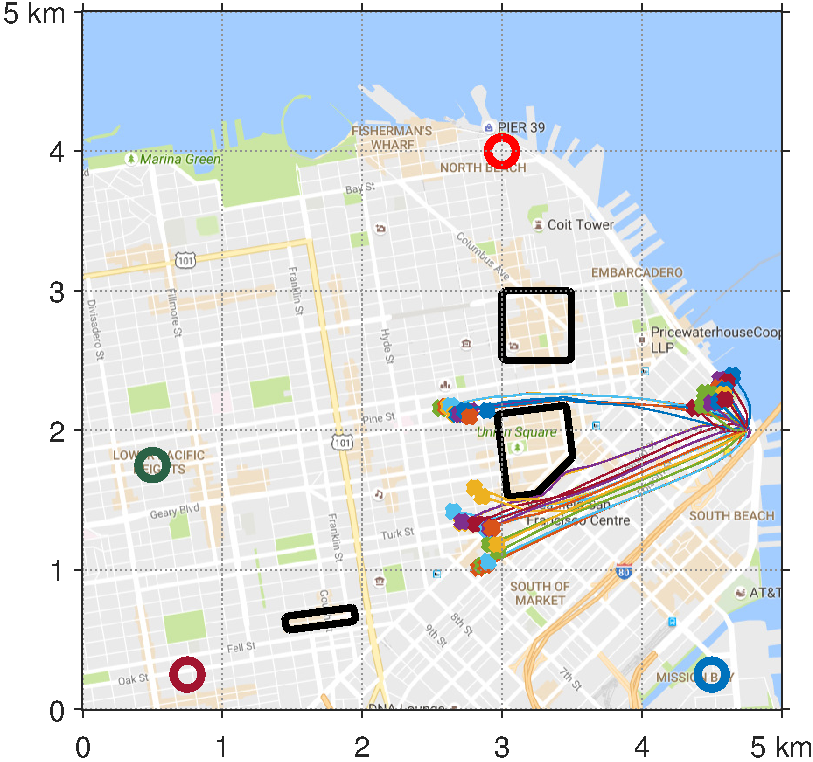
\includegraphics[width=\columnwidth]{figs/sf_d6sep0_s2}
  \subcaption{}
  \label{fig:sf_d6sep0_s2}
\end{subfigure}%

\begin{subfigure}{0.5\textwidth}
  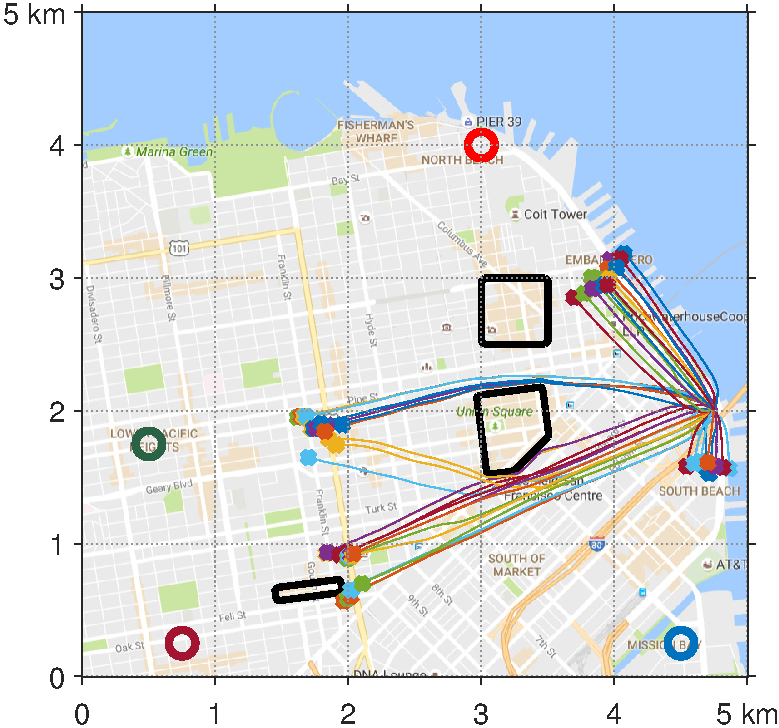
\includegraphics[width=\columnwidth]{figs/sf_d6sep0_s3}
  \subcaption{}
  \label{fig:sf_d6sep0_s3}
\end{subfigure}%
\begin{subfigure}{0.5\textwidth}
  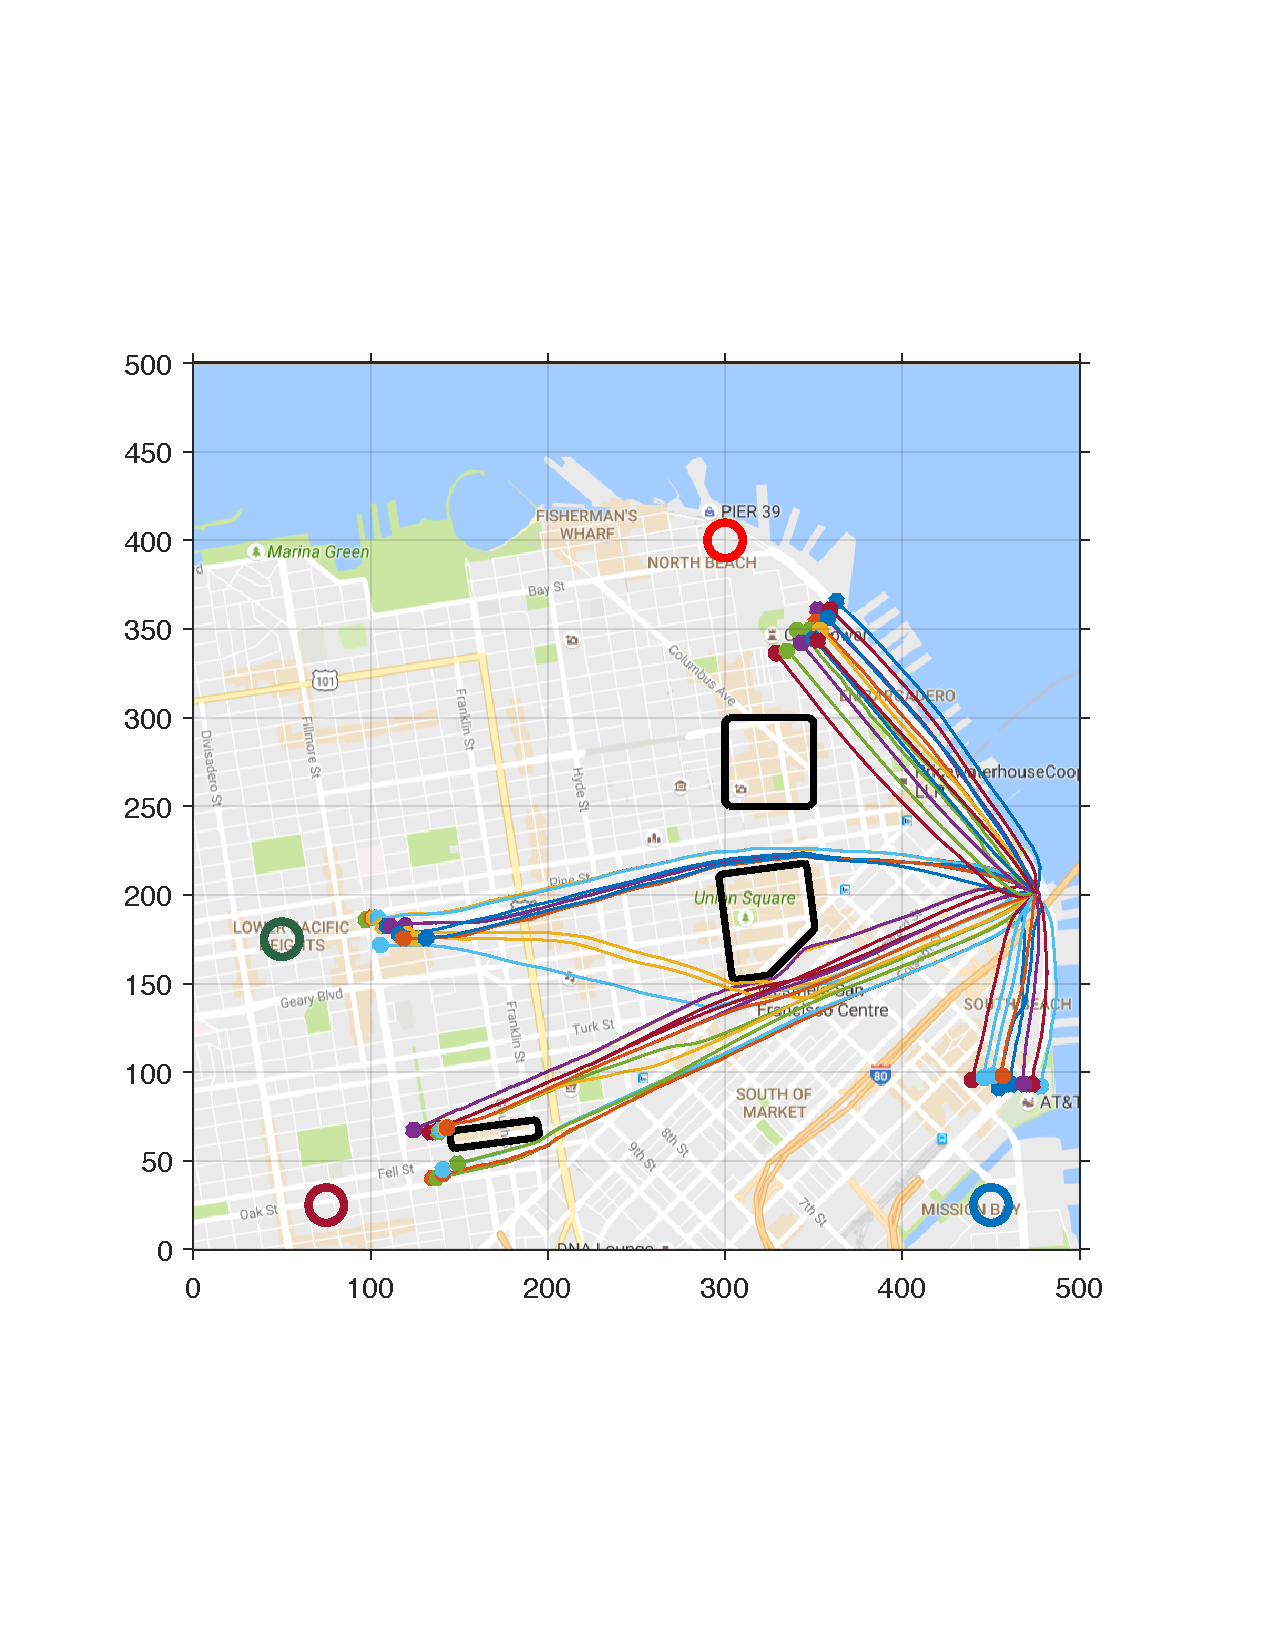
\includegraphics[width=\columnwidth]{figs/sf_d6sep0_s4}
  \subcaption{}
  \label{fig:sf_d6sep0_s4}
\end{subfigure}%
\caption{Snapshots of vehicle trajectories at different times for uniform disturbance with $d_{r} = 6$ m/s. The vehicles remain clear of all static obstacles despite the disturbance in the dynamics.}
\label{fig:trajectories_sf_snapshots}
\end{figure*}

The full trajectories of vehicles are shown in Figure \ref{fig:sf_d6sep0}. All vehicles reach their respective destinations. A zoomed-in version of Figure \ref{fig:sf_d6sep0} near the red target (Figure \ref{fig:sf_d6sep0_zoomed}) illustrates that vehicles are also outside each other's danger zones (circles around the vehicles) as required. 

\begin{figure*}
  \centering
  \begin{subfigure}{0.5\textwidth}
    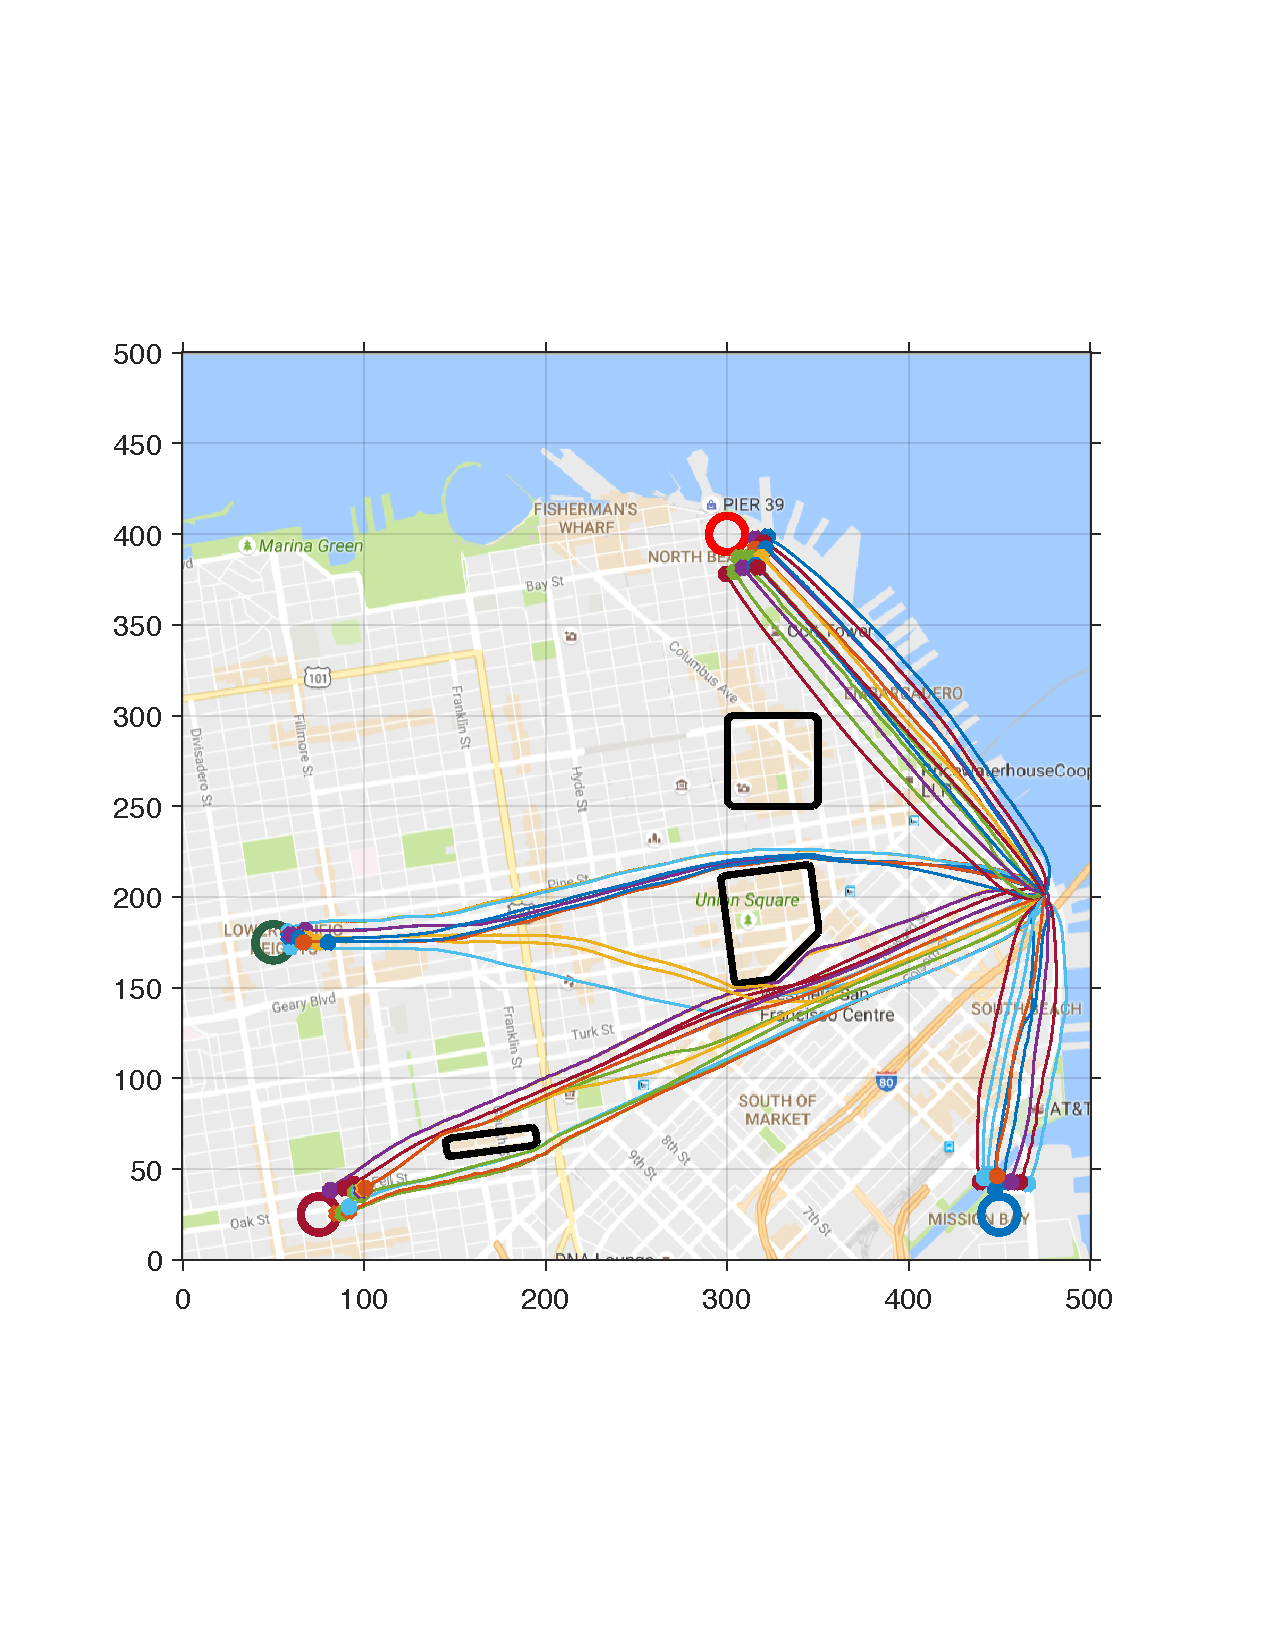
\includegraphics[width=\columnwidth]{figs/sf_d6sep0}
    \subcaption{Case-0: $d_r = 6m/s$, $\sta_i = 0$}
    \label{fig:sf_d6sep0}
  \end{subfigure}%
  \begin{subfigure}{0.5\textwidth}
    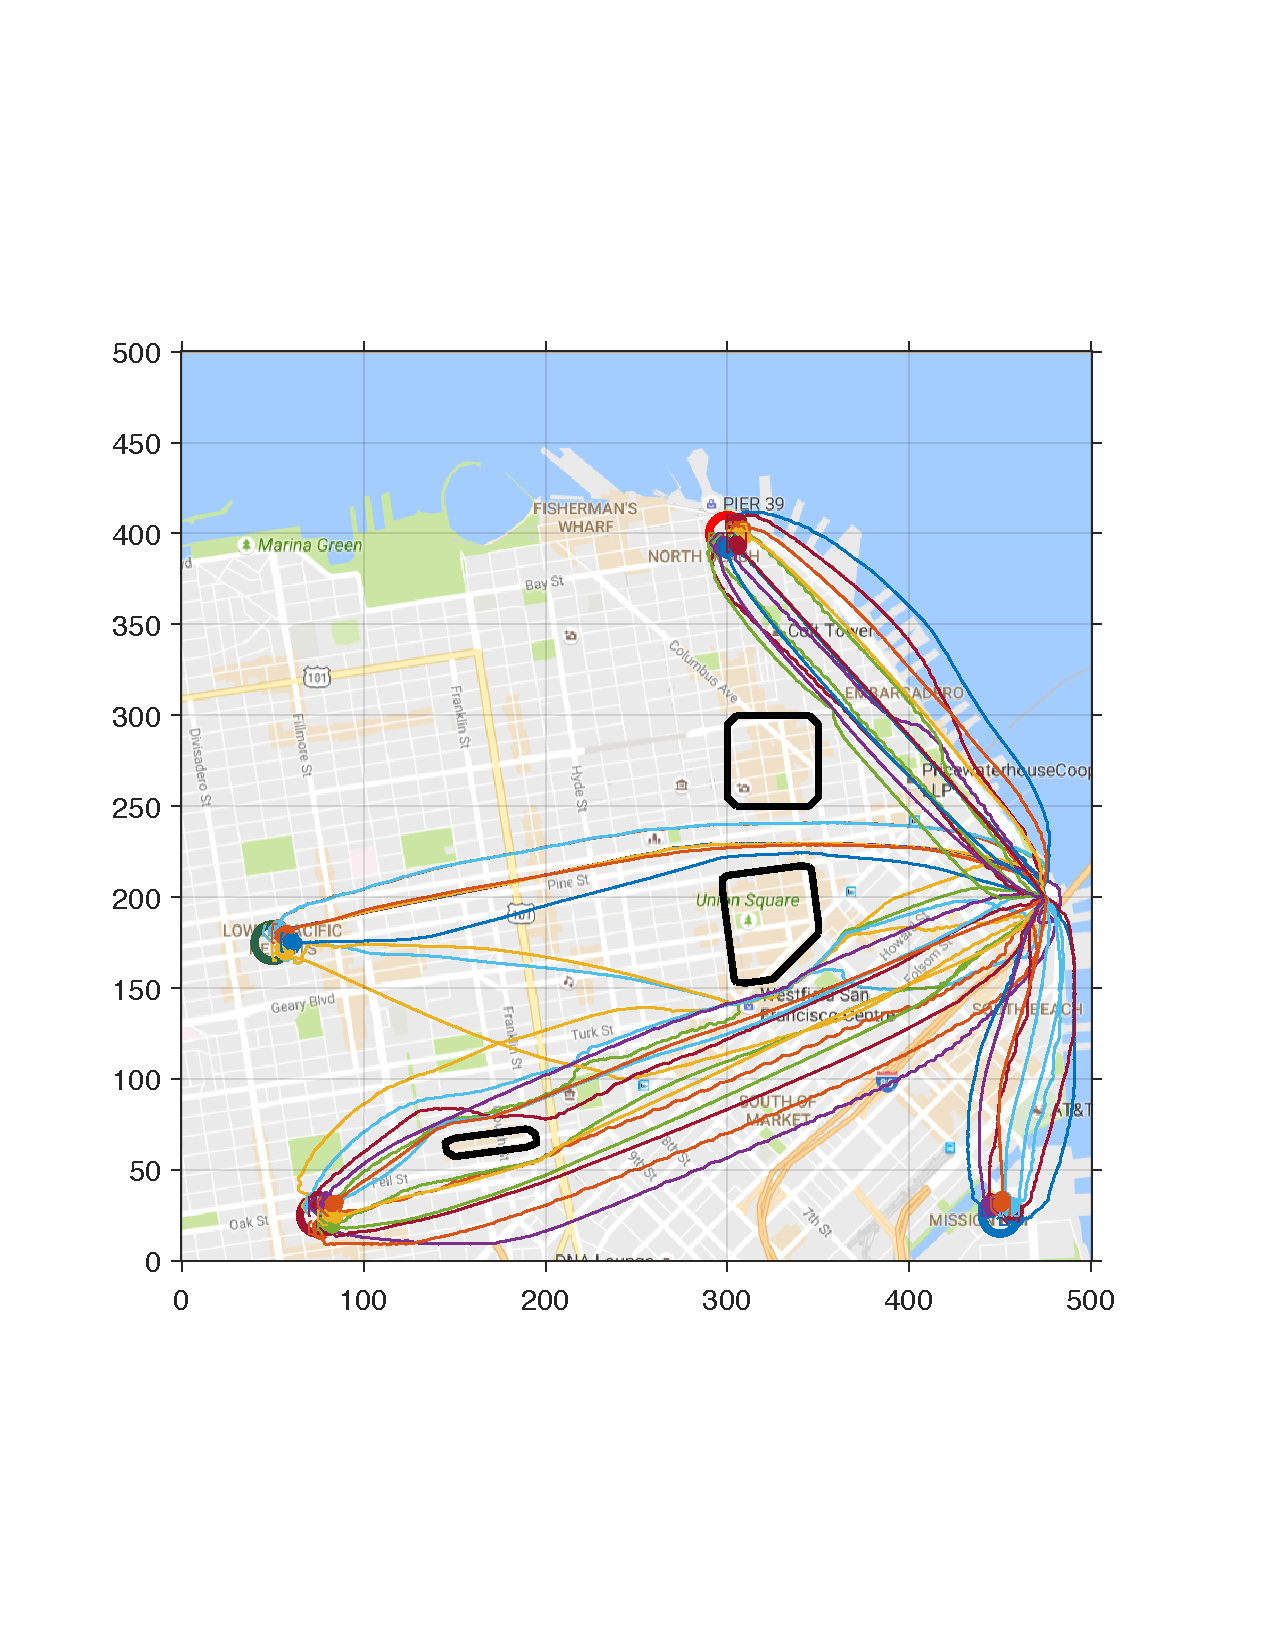
\includegraphics[width=\columnwidth]{figs/sf_d11sep0}
    \subcaption{Case-1: $d_r = 11m/s$, $\sta_i = 0$}
    \label{fig:sf_d11sep0}
  \end{subfigure}
  
  \begin{subfigure}{0.5\textwidth}
    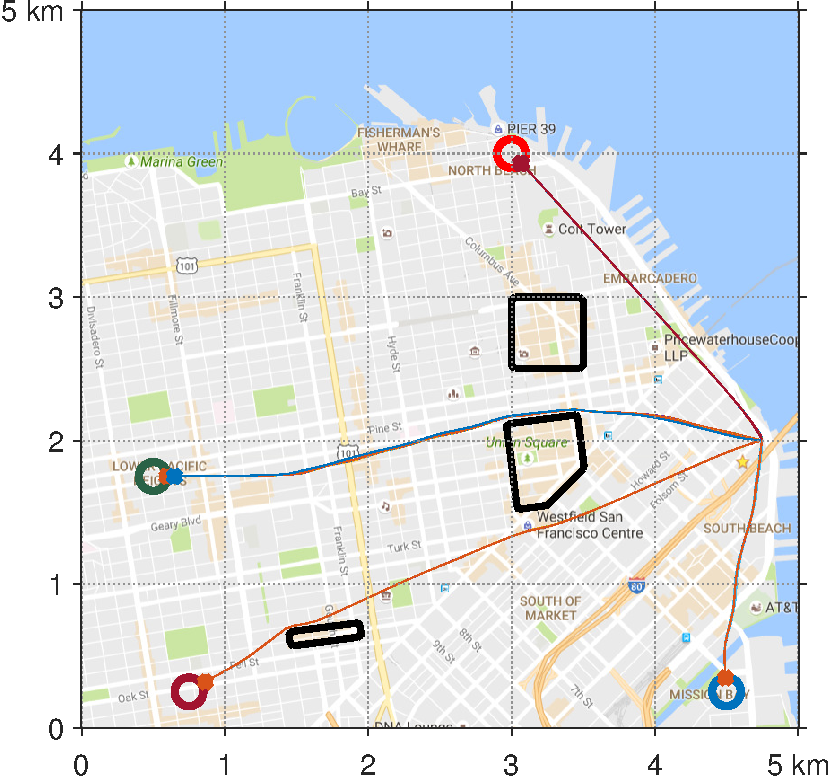
\includegraphics[width=\columnwidth]{figs/sf_d6sep5}
    \subcaption{Case-2: $d_r = 6m/s$, $\sta_i = 5(i-1)$}
    \label{fig:sf_d6sep5}
  \end{subfigure}%
  \begin{subfigure}{0.5\textwidth}
    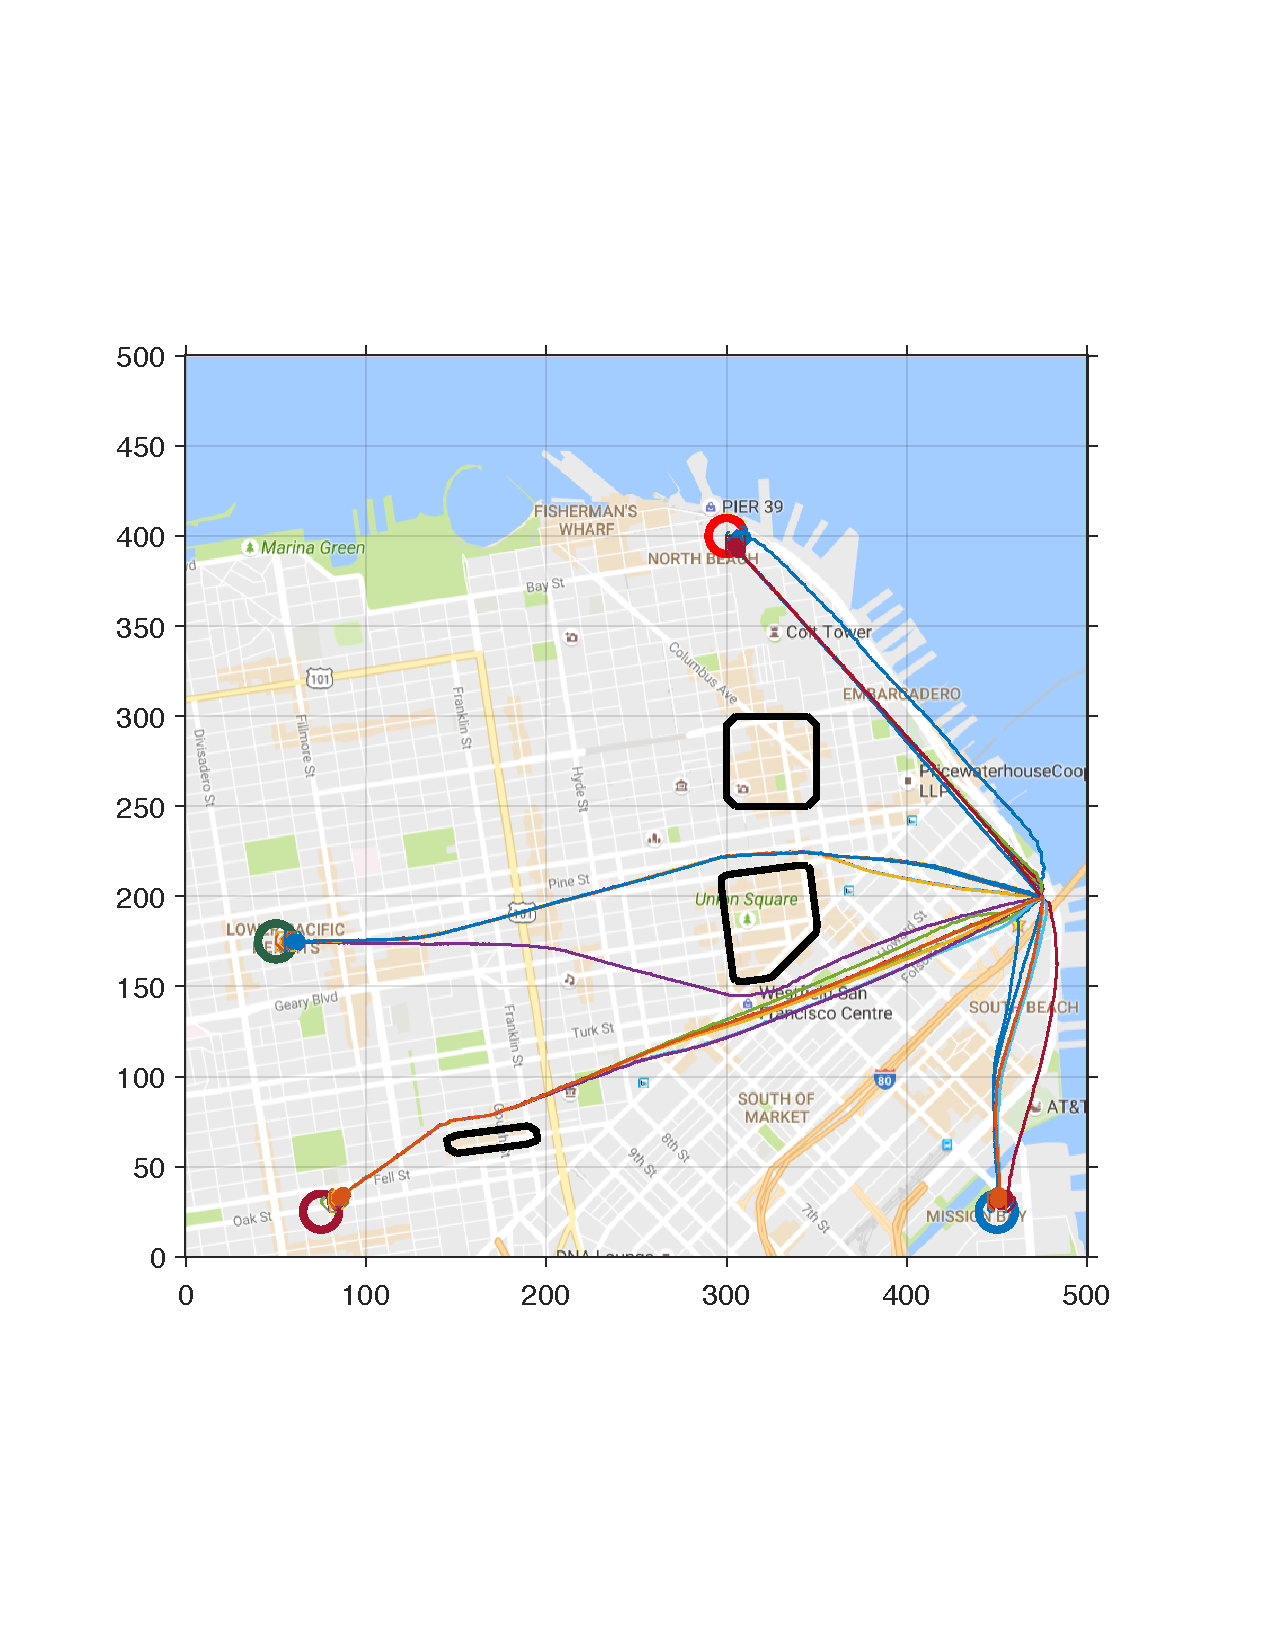
\includegraphics[width=\columnwidth]{figs/sf_d11sep5}
    \subcaption{Case-3: $d_r = 11m/s$, $\sta_i = 5(i-1)$}
    \label{fig:sf_d11sep5}
  \end{subfigure}
  \caption{Effect of the disturbance magnitude and the scheduled times of arrival on vehicle trajectories. All trajectories are simulated under uniformly random disturbance. The relative separation in the scheduled times of arrival of vehicles determines the number of lanes between a pair of origin and destination, and more and more tarjectories become time-separated as this relative separation increases. The disturbance magnitude determines the relative separation between different lanes, and more and more tarjectories become state-separated as the disturbance increases. }
  \label{fig:trajectories_sf}
\end{figure*}

\begin{figure}[h]
  \centering
  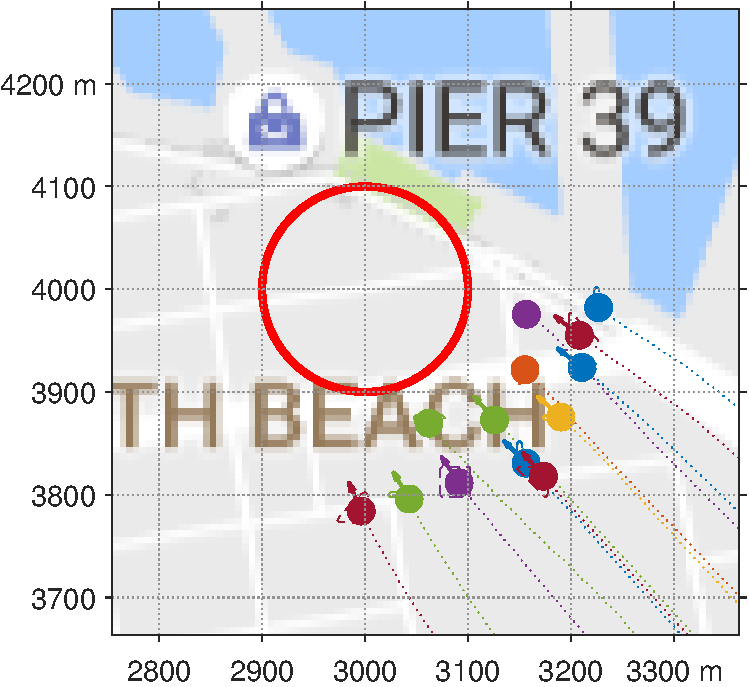
\includegraphics[width=\columnwidth]{figs/sf_d6sep0_zoomed}
  \caption{Zoomed-in version of vehicle trajectories near the red target in Figure \ref{fig:sf_d6sep0}. The STP algorithm ensures that the vehicles are outside each other's danger zones (circles around the vehicles).} 
  \label{fig:sf_d6sep0_zoomed}
\end{figure}
It is interesting to note that the vehicles going to the same destination take different trajectories. This is because all vehicles have same scheduled time of arrival, and hence the lower-priority vehicles do not have the flexibility to wait for the higher-priority vehicles. In order to ensure that they reach their destinations on time, they take alternative trajectories to their destinations, forming different ``traffic lanes''. Thus, the vehicles' trajectories obtained in this case are predominately \textit{state-separated} trajectories, i.e., they follow different state trajectories but at the same time. 

Although the plotted trajectories in Figure \ref{fig:sf_d6sep0} are for a particular realization of the (uniformly random) disturbances, the STP algorithm guarantees obstacle avoidance regardless of the realized disturbance. To illustrate this, we plot the trajectories of a particular vehicle ($\veh_{17}$) for three different disturbance realizations -- uniform, worst-case, and constant wind from the west direction -- in Figure \ref{fig:dstb_trajs}. One can see that the trajectories are nearly indistinguishable even in the zoomed-in plot on the right. 

\begin{figure*}[!htb]
  \centering
  \begin{subfigure}{0.5\textwidth}
    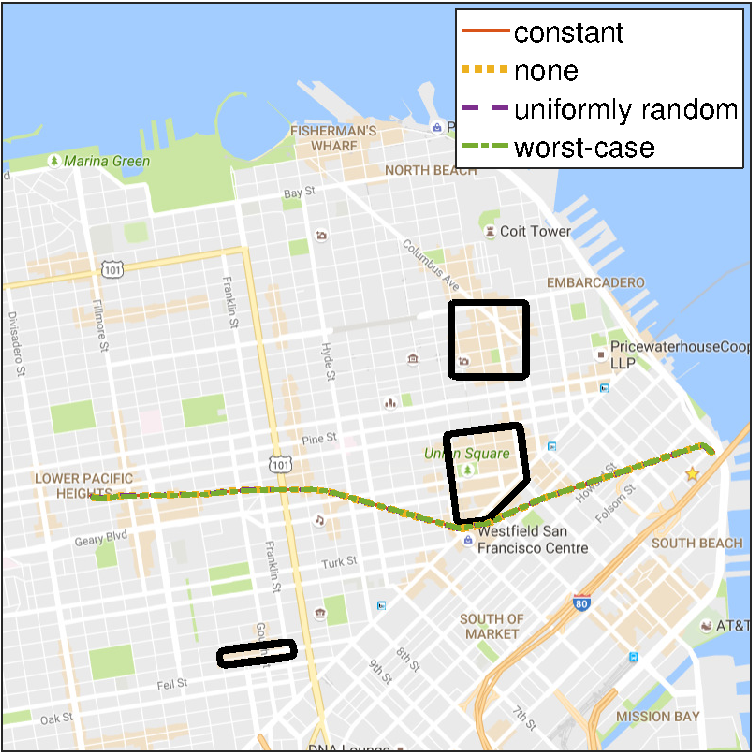
\includegraphics[width=\columnwidth]{figs/dstb_trajs}
    \subcaption{}
    \label{fig:dstb_trajs_s1}
  \end{subfigure}%
  \begin{subfigure}{0.5\textwidth}
    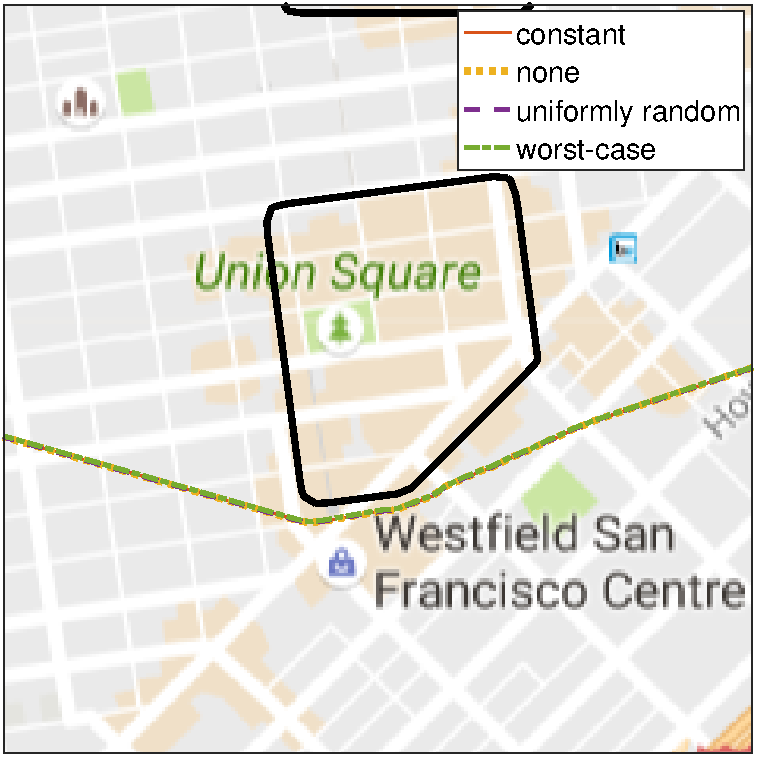
\includegraphics[width=\columnwidth]{figs/dstb_trajs_zoomed_in}
    \subcaption{}
    \label{fig:dstb_trajs_s2}
  \end{subfigure}%

  \caption{Trajectories of $\veh_{17}$ under different types of bounded disturbances -- constant wind from the west, no wind, uniformly random wind, and worse-case wind. The right plot zooms in on the beginning of the left plot.}
  \label{fig:dstb_trajs}
\end{figure*}

Figure \ref{fig:min_dists} shows the minimum distance between $\veh_{17}$ and other vehicles. One can see that this distance is never below $10$ m, which is the minimum required separation between the vehicles. The separation distance is small in the beginning because the vehicles need to depart as soon as possible while maintaining this minimum required separation. 

\begin{figure*}[!htb]
  \centering
  \begin{subfigure}{0.5\textwidth}
    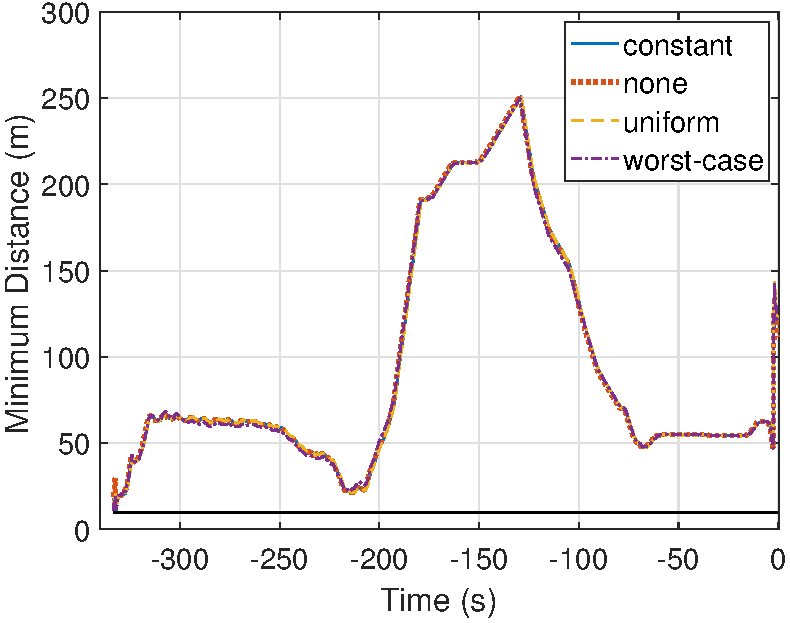
\includegraphics[width=\columnwidth]{figs/min_dists}
    \subcaption{}
    \label{fig:min_dists_s1}
  \end{subfigure}%
  \begin{subfigure}{0.5\textwidth}
    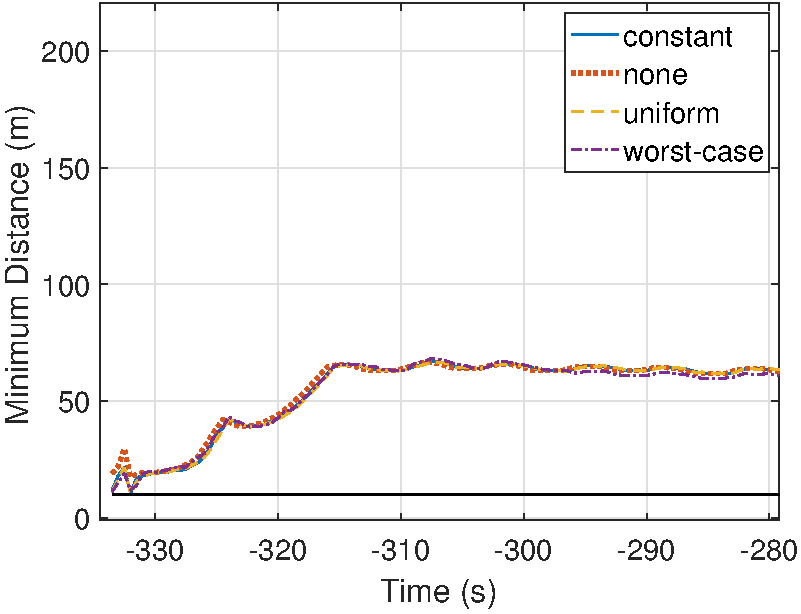
\includegraphics[width=\columnwidth]{figs/min_dists_zoomed_in}
    \subcaption{}
    \label{fig:min_dists_s2}
  \end{subfigure}%
  
  \caption{Minimum distance to other vehicles for $\veh_{17}$ under different types of bounded disturbances -- constant wind from the west, no wind, uniformly random wind, and worse-case wind. The right plot zooms in on the beginning of the left plot.}
  \label{fig:min_dists}
\end{figure*}

Figure \ref{fig:reactivity} shows the optimal control action in terms of the turn rate and the linear speed of each vehicle, demonstrating that the tracking control law reacts to tracking error due to disturbances in an intuitive way. Both subplots show the control law when the vehicle is facing east. Figure \ref{fig:Wcontrol} indicates, for example, that generally when the tracking error is such that the vehicle is too far to the right compared to the nominal position, the optimal tracking control is to turn left. Figure \ref{fig:Vcontrol} indicates, for example, that when the vehicle is too far ahead of the nominal position, it should slow down. The optimal turn rate and linear speed controls ensure that the vehicle never deviates from the nominal trajectory for more than $5$ m.

\begin{figure*}[!htb]
  \centering
  \begin{subfigure}{0.5\textwidth}
    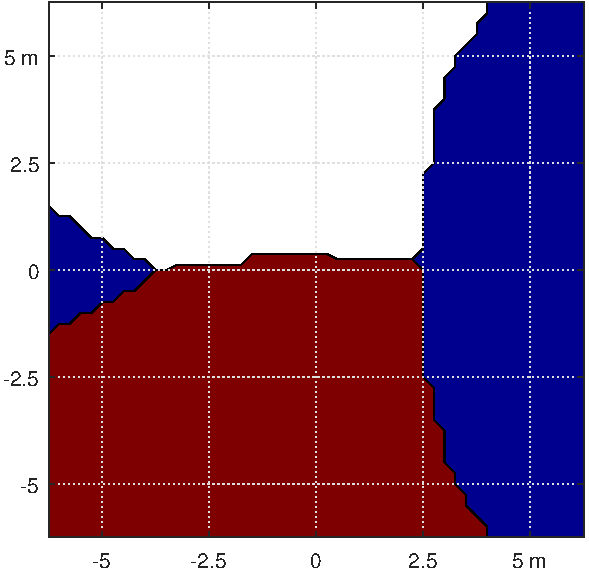
\includegraphics[width=\columnwidth]{figs/Wcontrol}
    \subcaption{Turn rate control as a function of tracking error. White: turn right; red: turn left; blue: go straight.}
    \label{fig:Wcontrol}
  \end{subfigure}%
  \begin{subfigure}{0.5\textwidth}
    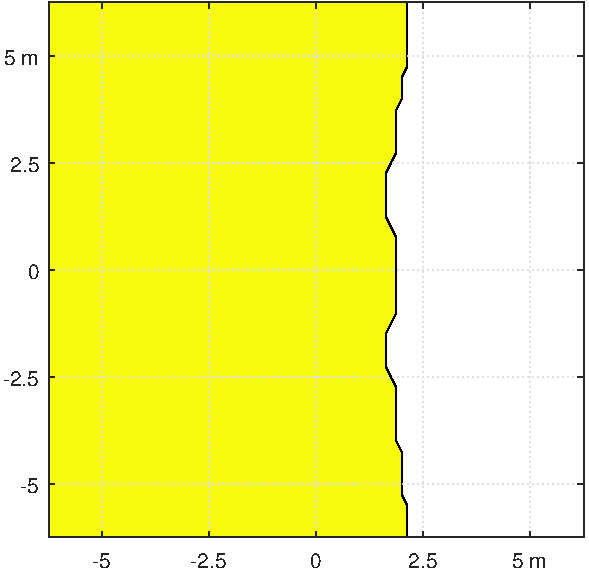
\includegraphics[width=\columnwidth]{figs/Vcontrol}
    \subcaption{Linear speed control as a function of tracking error. Yellow: high speed; white: low speed.}
    \label{fig:Vcontrol}
  \end{subfigure}%
  
  \caption{Optimal tracking control law for each vehicle for a heading of zero degrees (facing towards the right).}
  \label{fig:reactivity}
\end{figure*}

The average trajectory computation time per vehicle is 2 seconds using a CUDA implementation of the level set toolbox on a desktop computer with a Core i7 5820K processor and two GeForce GTX Titan X graphics processing units. Note that all this computation is done offline and the resulting optimal policy $\tracklaw_j(e_j)$ is obtained as a lookup table. In real time, neither any computation nor any communication between vehicles is required. Only a lookup table query is required, and this can be performed very quickly in real time. This illustrates the capability of STP as a provably safe trajectory planning algorithm for large multi-vehicle systems. Without CUDA, the computation time per vehicle is 33 seconds using a C++ implementation of the level set toolbox, and 200 seconds using a MATLAB implementation.